% Set spellcheck for TexStudio
%!TeX spellcheck = en_US
%!TeX root = ../thesis.tex
\mainmatter
\appendix
\chapter{Additional plots from Benchmark}
\begin{figure}[H]
	\centering
	\begin{subfigure}[htpb]{0.3\textwidth}
		\centering
		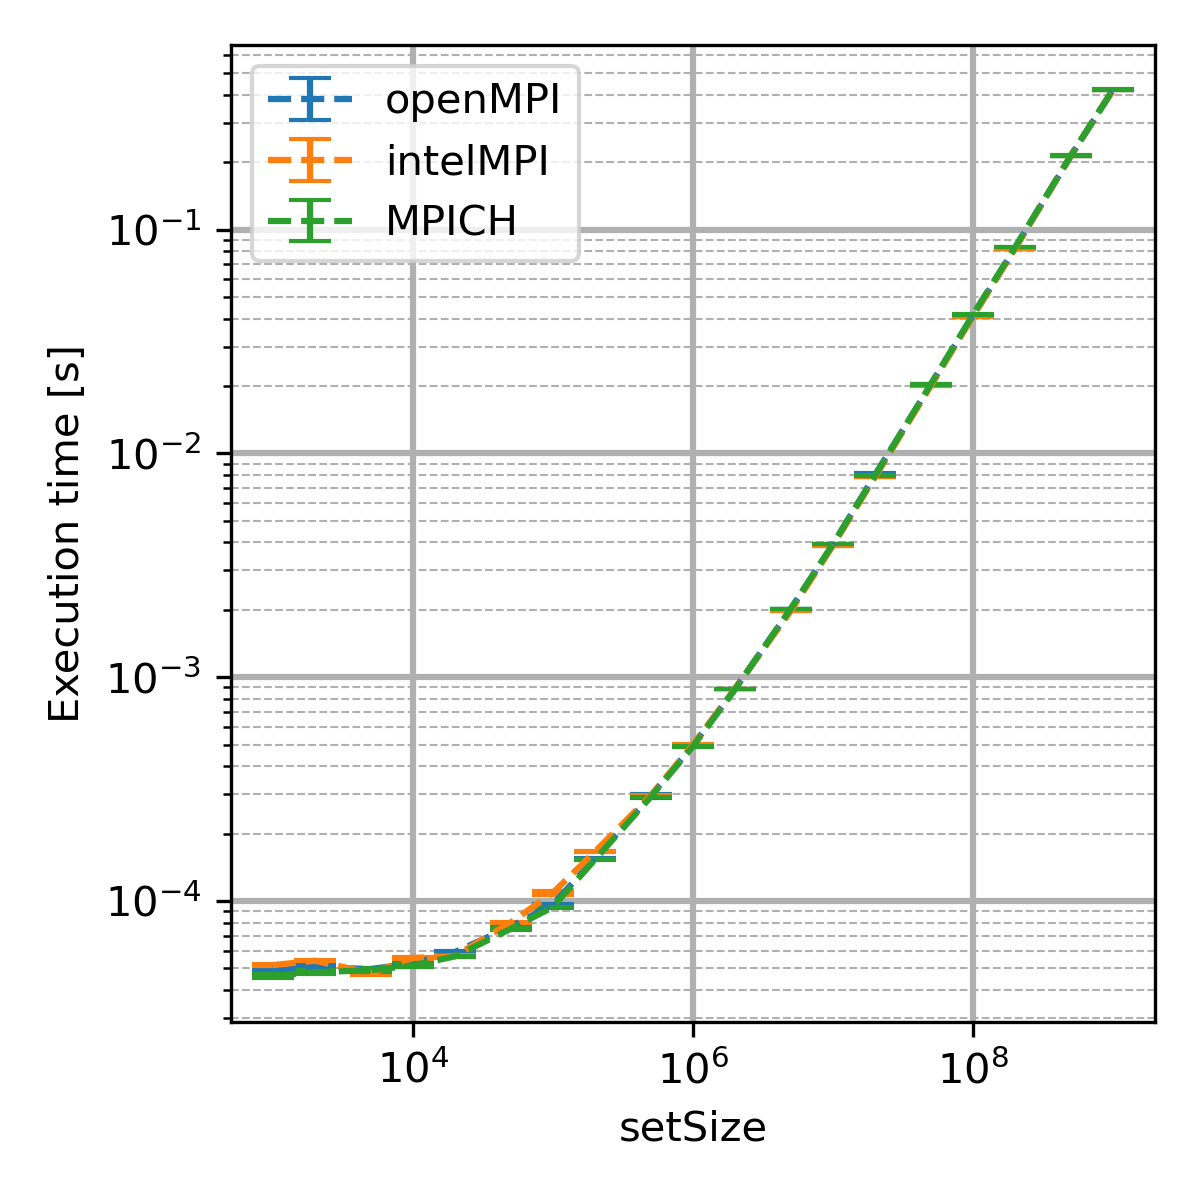
\includegraphics[width=\textwidth]{../plots/AllreduceLibsButterfly/32x32AllreduceLibsButterfly.png}
		\caption{\texttt{All\-re\-duce\_But\-ter\-fly} on $p=(32\times32)$}
	\end{subfigure}
	\hfill
	\begin{subfigure}[htpb]{0.3\textwidth}
		\centering
		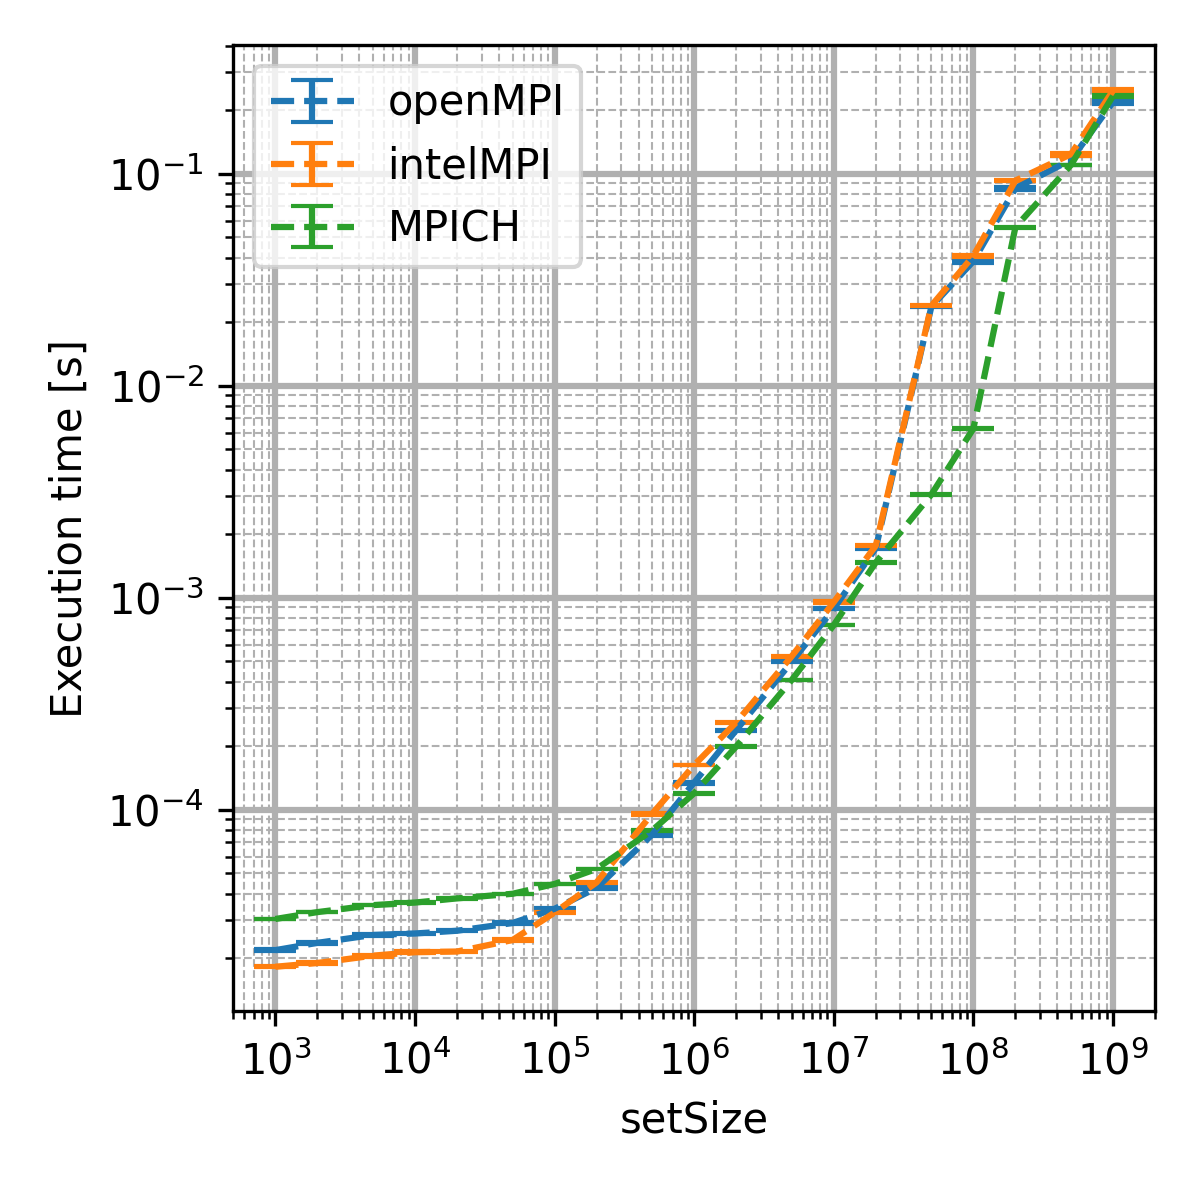
\includegraphics[width=\textwidth]{../plots/AllreduceLibsButterflyReverse/32x1AllreduceLibsButterflyReverse.png}
		\caption{\texttt{All\-re\-duce\_But\-ter\-fly \_Reversed} on $p=(32\times1)$}
		\label{fig:AllreduceFoundationLibsAppendix32x1}
	\end{subfigure}
	\hfill
	\begin{subfigure}[htpb]{0.3\textwidth}
		\centering
		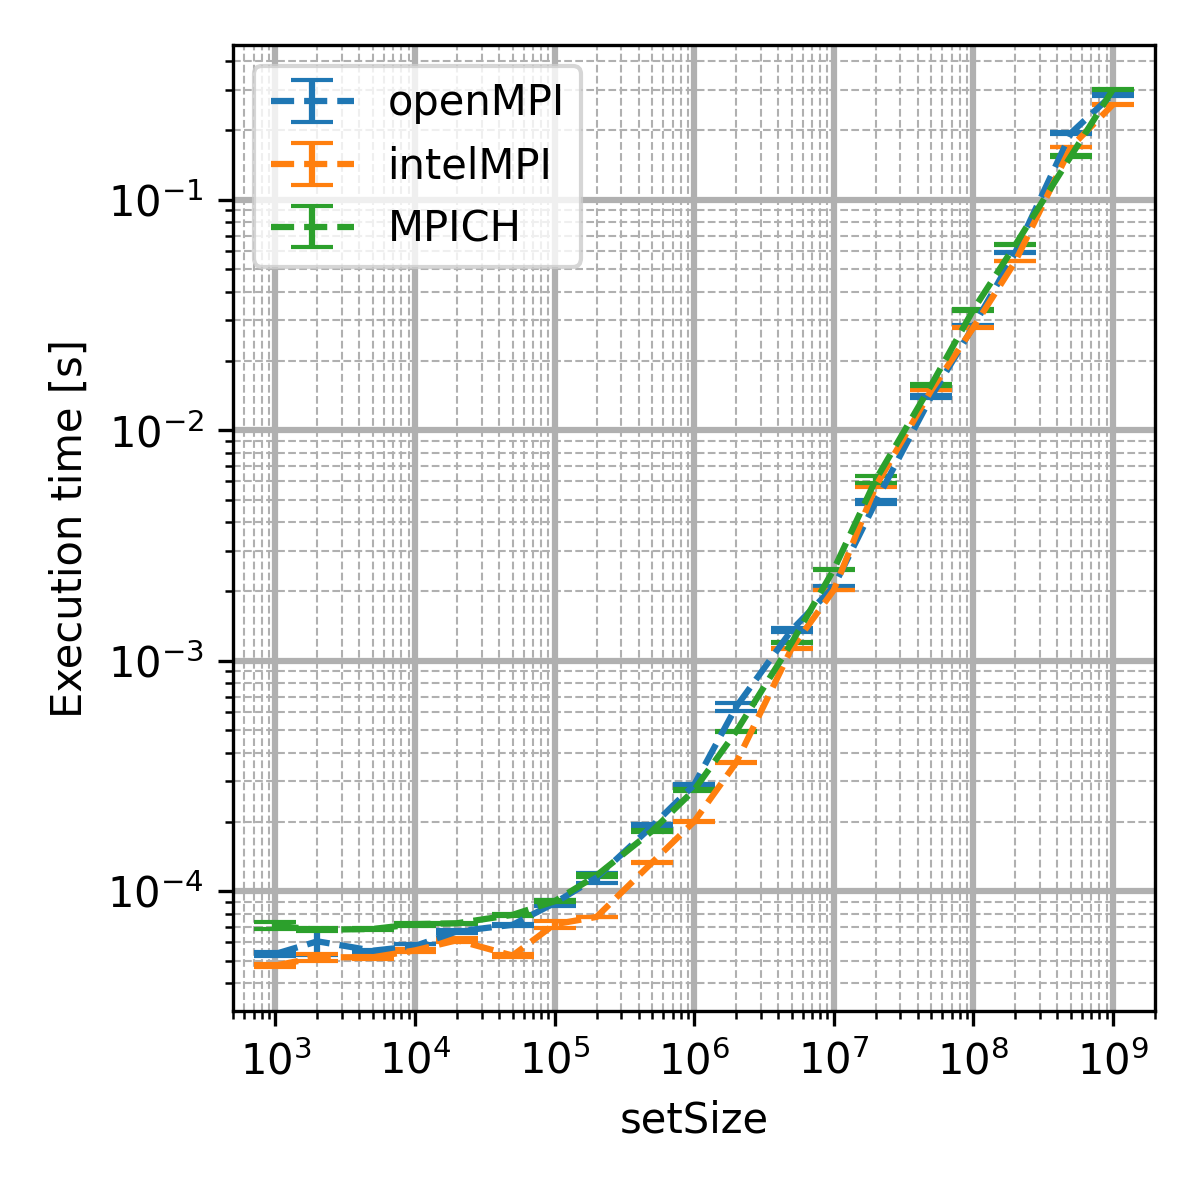
\includegraphics[width=\textwidth]{../plots/AllreduceLibsButterflyReverse/32x32AllreduceLibsButterflyReverse.png}
		\caption{\texttt{All\-re\-duce\_But\-ter\-fly \_Reversed} on $p=(32\times32)$}
	\end{subfigure}
	
	\vspace{3mm}
	\hspace*{\fill}
	\begin{subfigure}[htpb]{0.3\textwidth}
		\centering
		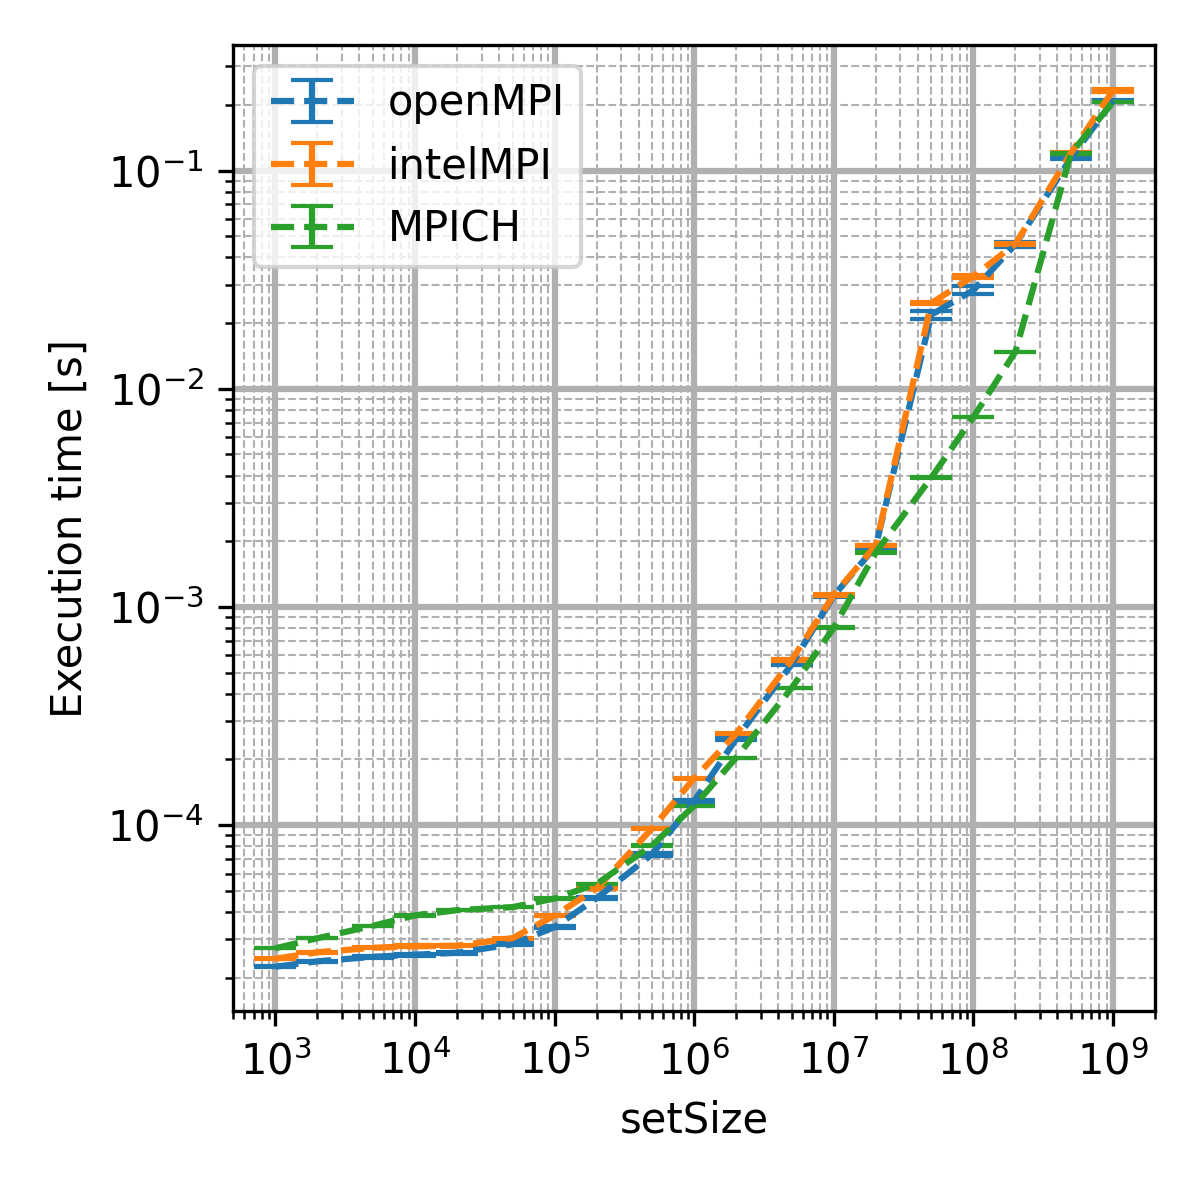
\includegraphics[width=\textwidth]{../plots/AllreduceLibsShift/34x1AllreduceLibsShift.png}
		\caption{\texttt{All\-re\-duce\-\_Shift} on $p=(34\times1)$}
		\label{fig:AllreduceFoundationLibsAppendix34x1}
	\end{subfigure}
	\hfill
	\begin{subfigure}[htpb]{0.3\textwidth}
		\centering
		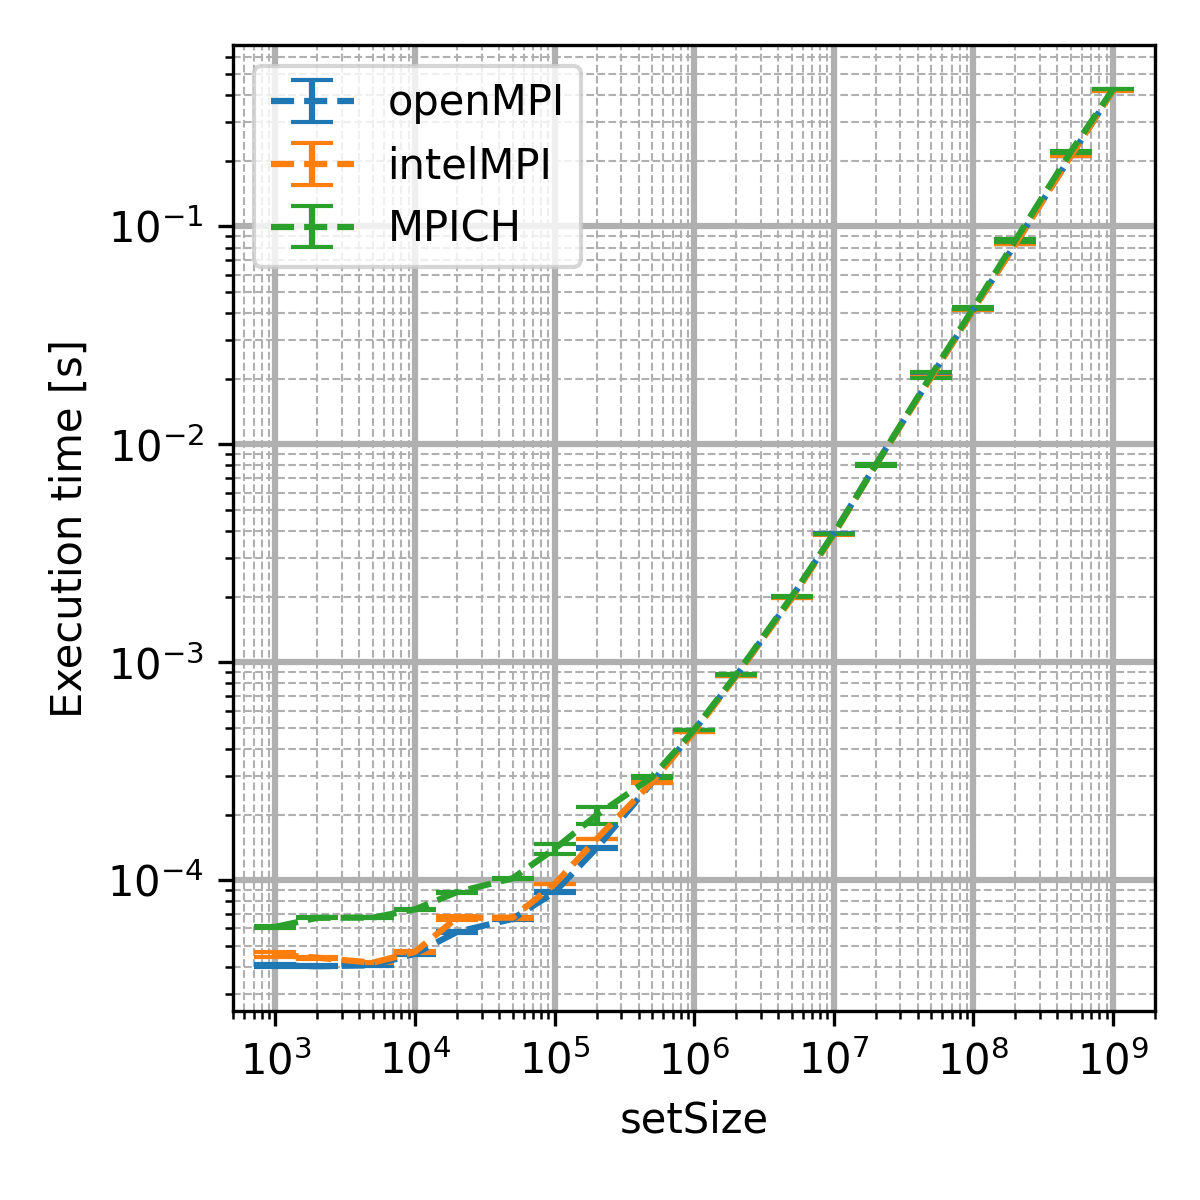
\includegraphics[width=\textwidth]{../plots/AllreduceLibsShift/34x32AllreduceLibsShift.png}
		\caption{\texttt{All\-re\-duce\-\_Shift} on $p=(34\times32)$}
	\end{subfigure}
	\hspace*{\fill}

	\caption{Benchmark of the three foundation Allreduce implementations (\texttt{All\-re\-duce\_But\-ter\-fly}, \texttt{All\-re\-duce\_But\-ter\-fly\_Reversed} and \texttt{All\-re\-duce\-\_Shift}). The influence of using different MPI libraries is tested. Execution time $t$ is plotted against set size $|\Tilde{S}|$. The different processor layouts are indicated by $p$.}
	\label{fig:AllreduceFoundationLibsAppendix}
\end{figure}


\begin{figure}[ht]
	\centering
	\begin{subfigure}[b]{0.4\textwidth}
		\centering
		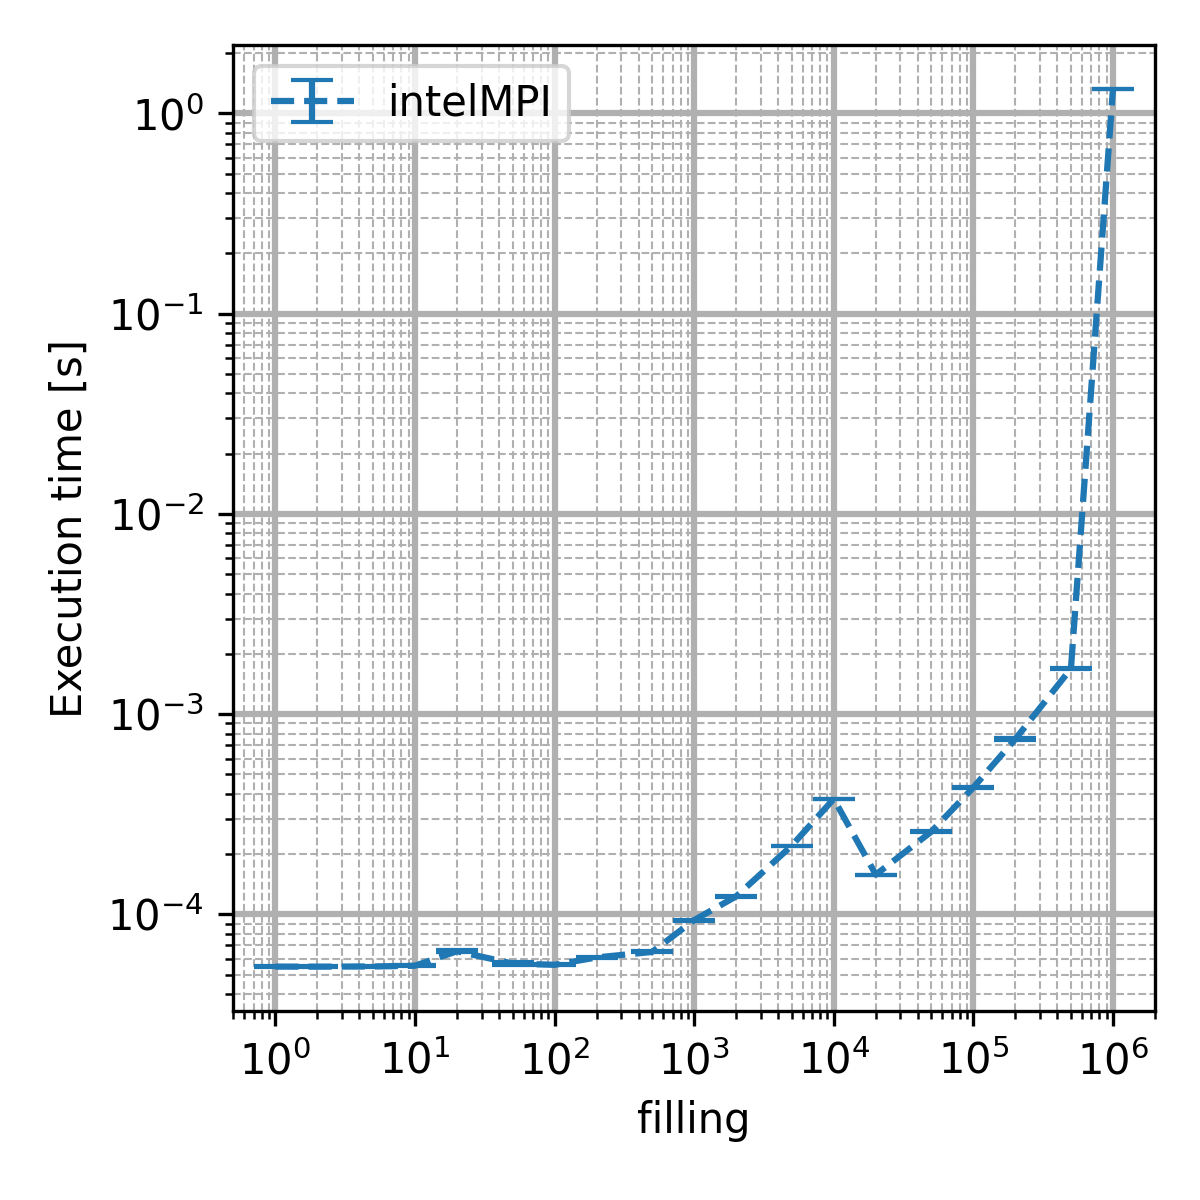
\includegraphics[width=\textwidth]{../plots/AllgatherIntelMPIConcentrated/32x32AllgatherIntelMPIConcentrated.png}
		\caption{$p=(32\times32)$}
	\end{subfigure}
	\hfill
	\begin{subfigure}[b]{0.4\textwidth}
		\centering
		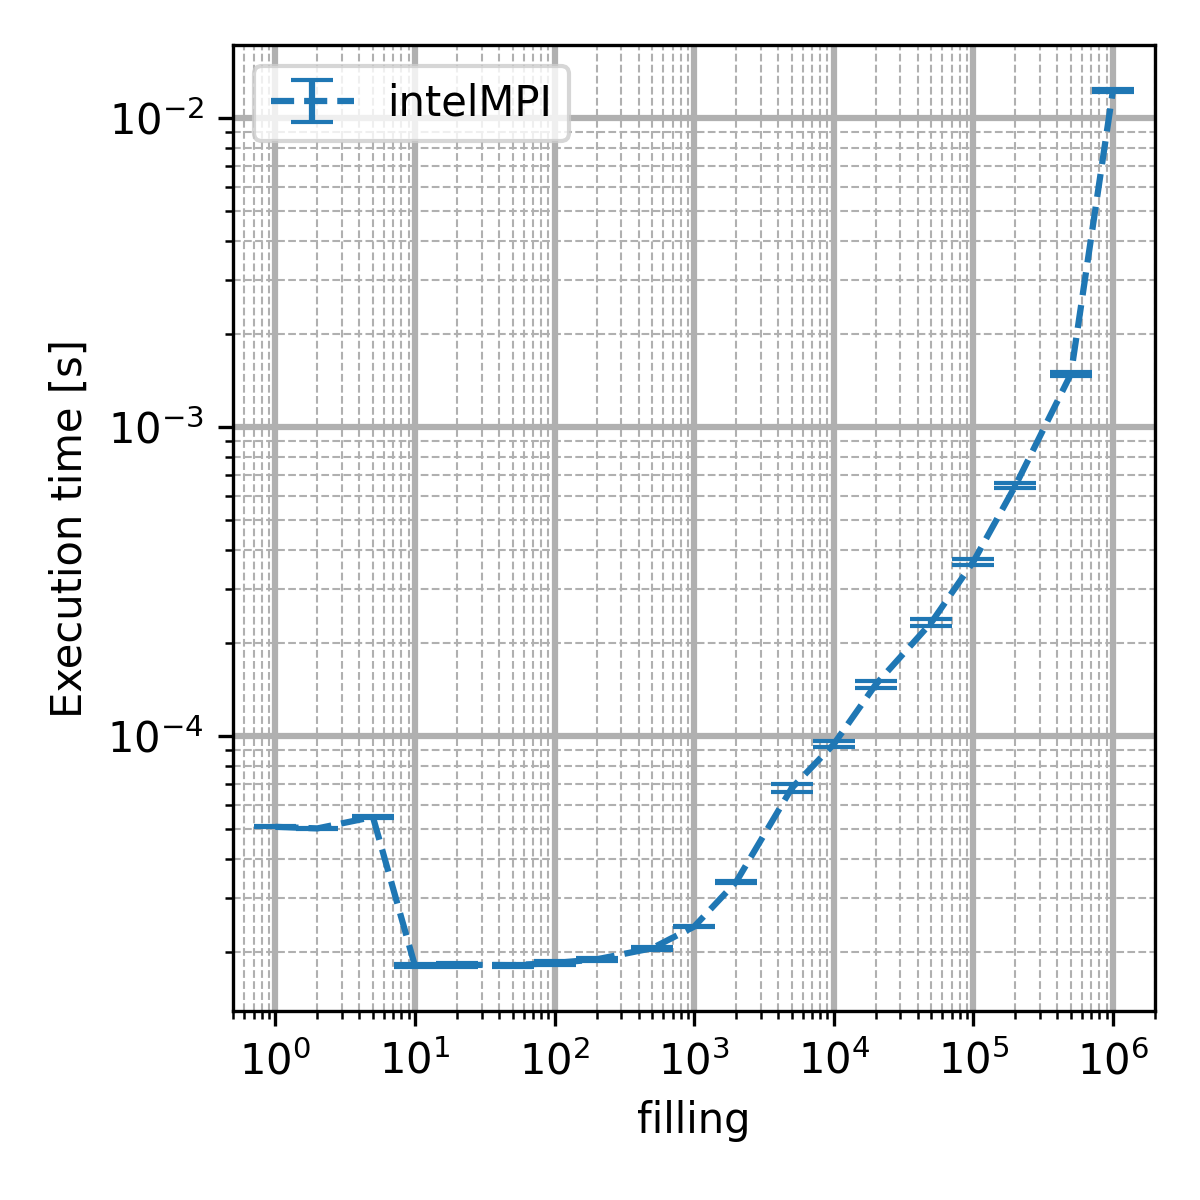
\includegraphics[width=\textwidth]{../plots/AllgatherIntelMPIConcentrated/32x1AllgatherIntelMPIConcentrated.png}
		\caption{$p=(32\times1)$}
	\end{subfigure}
	\vspace{5mm}
	\begin{subfigure}[b]{0.4\textwidth}
		\centering
		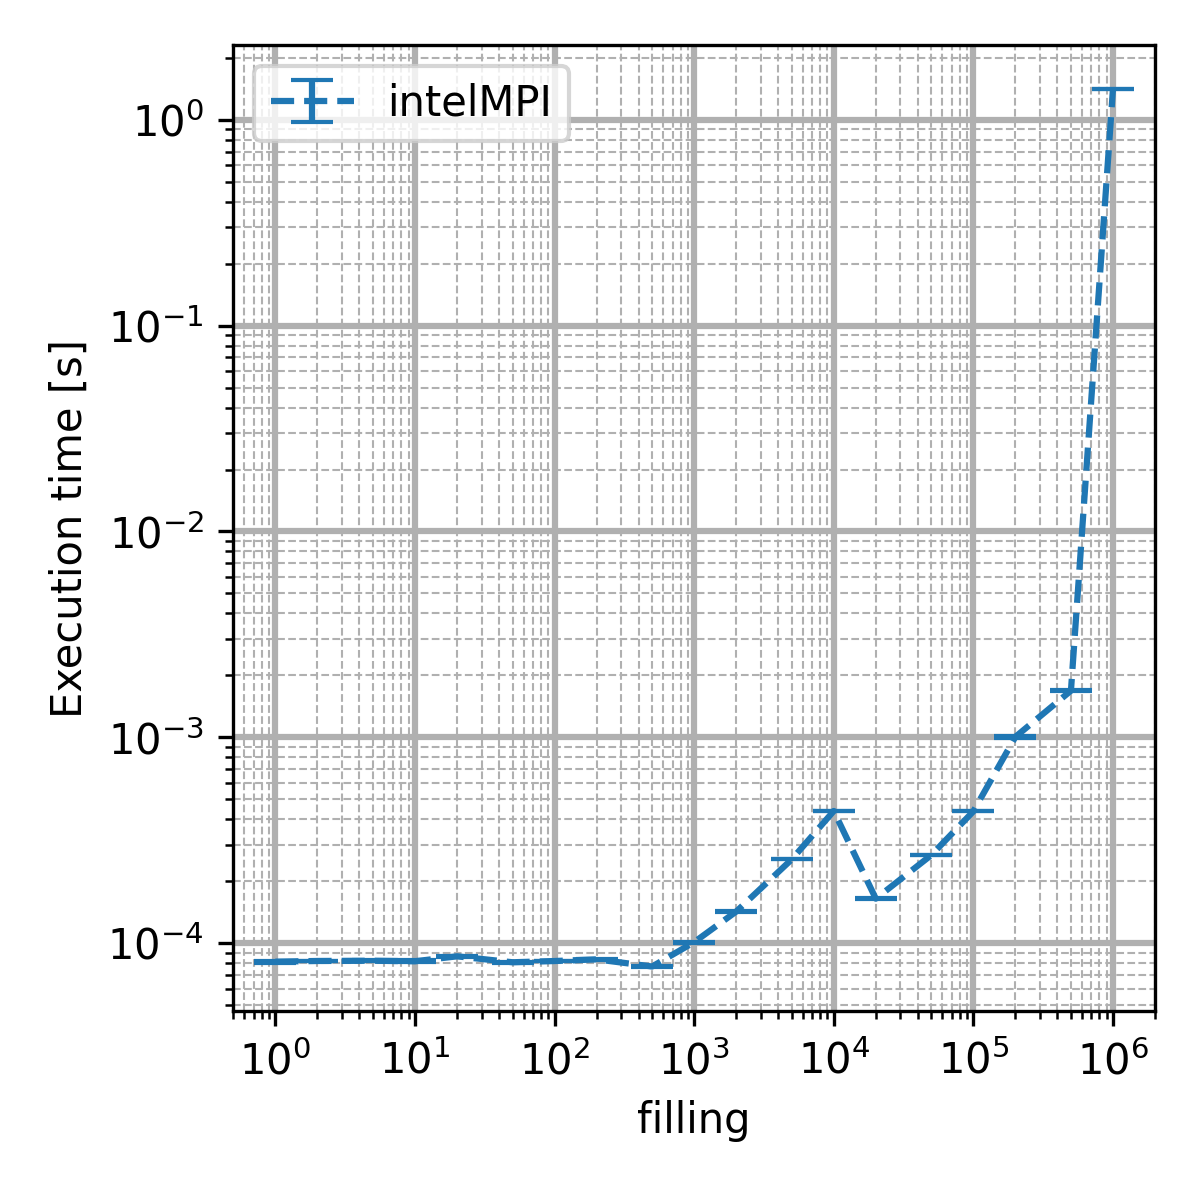
\includegraphics[width=\textwidth]{../plots/AllgatherIntelMPIConcentrated/34x32AllgatherIntelMPIConcentrated.png}
		\caption{$p=(34\times32)$}
	\end{subfigure}
	\hfill
	\begin{subfigure}[b]{0.4\textwidth}
		\centering
		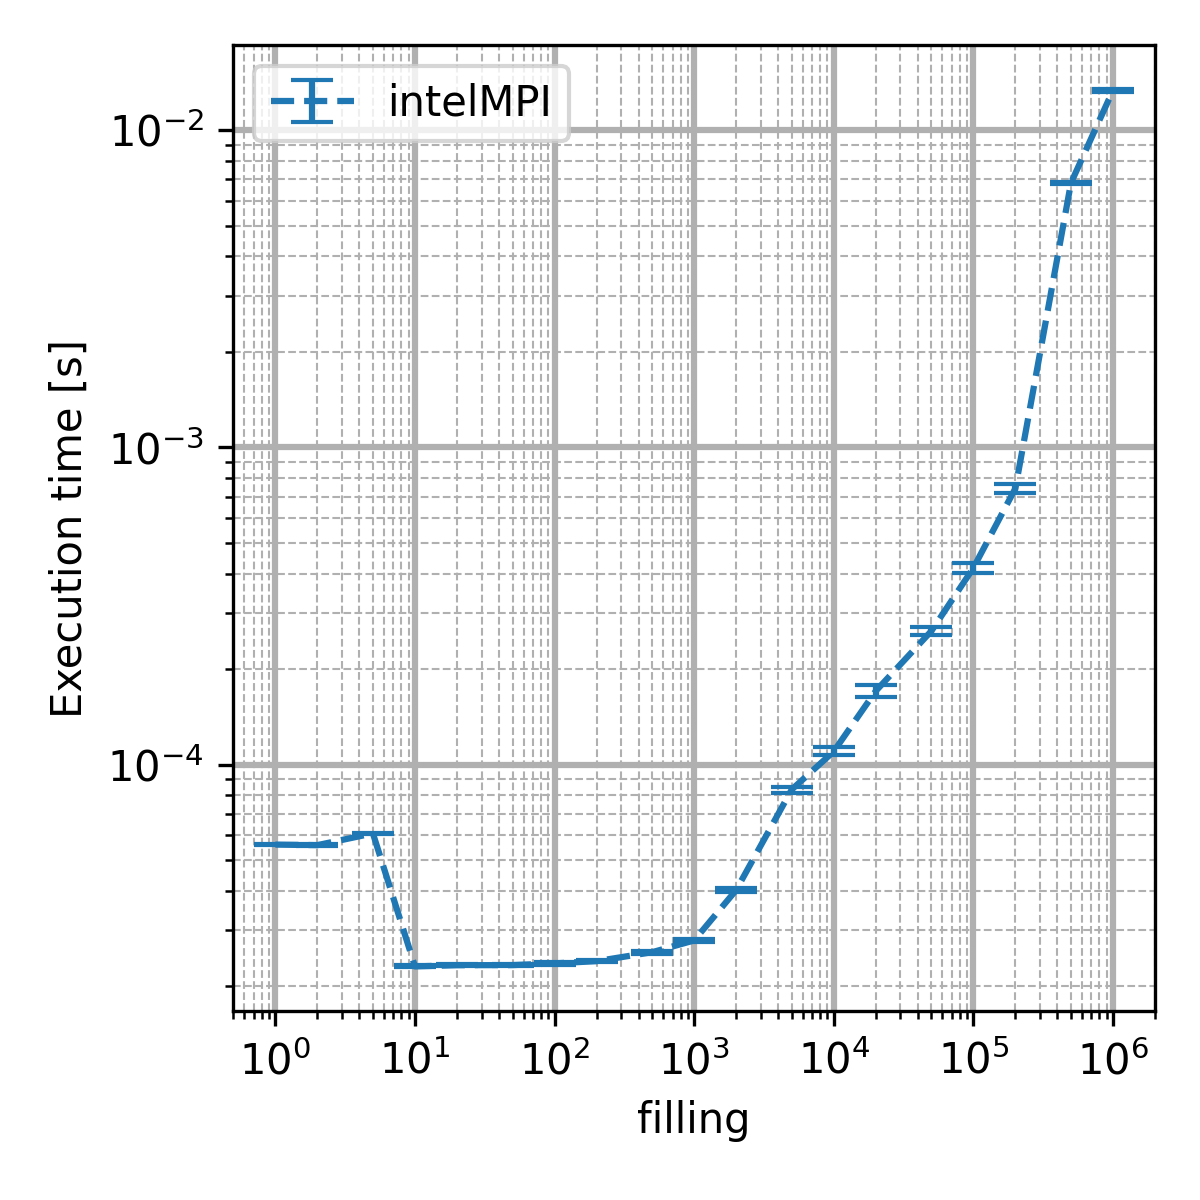
\includegraphics[width=\textwidth]{../plots/AllgatherIntelMPIConcentrated/34x1AllgatherIntelMPIConcentrated.png}
		\caption{$p=(34\times1)$}
	\end{subfigure}
	\caption{Performance of the native IntelMPI Allgather. Execution time $t$ is plotted against set filling $\Phi$. All elements are held by one only process before the Allgather.}
	\label{fig:AllgatherIntelMPIConcentrated}
\end{figure}







